%%% -*-LaTeX-*-

\chapter{SAT Encodings}

In this chapter we'll examine how the language forms we saw in the previous chapter are efficiently encoded as boolean formulas. A program in SweetPea is translated to a boolean formula in Conjunctive Normal Form (CNF), which is a canonicalization that is frequently used by SAT solvers and samplers. We use two techniques for efficient SAT encodings: we encode large "counting" constraints using a Tsietin transform, and user's derivation constraints more directly. After examining how a program is encoded, we'll also discuss the runtime communication with the sampler, and why the correctness guarantees are preserved.

\section{Conjunctive Normal Form (CNF)}

A boolean formula consists of boolean variables combined using boolean operators, such as AND, OR and NOT. There are many canonical forms for boolean formulas; the one that SAT solvers commonly use is Conjunctive Normal Form (CNF). CNF is an "and of ors". This means that CNF is built out of OR clauses, which are clauses in which the boolean OR operator is applied to a list of variables. A or B or (not C) or D is an example of an OR clause. CNF is then the AND operator applied to a list of OR clauses. (A or B) and (C or not D) is an example of a boolean formula in CNF.

SAT solvers typically process boolean formulas in CNF. This is partially because they are amenable to the search strategies that solvers commonly employ while searching for satisfying assignments, and partially because there is an efficient translation from a boolean formula in any form to the CNF canonical form.

More specifically, solvers typically process boolean formulas in the DIMACS CNF form. In the DIMACS convention, boolean variables are denoted by their index, and negation is denoted by a minus sign. This means that a formula like (A or B) and (C or not D) is represented as (1 or 2) and (3 or -4). This index based renaming is very convinient as a convention for generating fresh variable names-- you just need to increment the variable counter to get a fresh variable. Each or-clause is written on an individual line, and every term within the or-clause is written as an element of a list; each list is terminated with the number 0. Finally, each formula also has a header which clues the consumer to the number of variables and clauses in formula. The full DIMACS CNF specification of the example in this paragraph is:
p cnf 4 2
1, 2, 0
3, -4, 0

This specification is the langauge required to leverage the awesome power of SAT samplers and solvers, but it is clearly not amemable to being manually specified by human hands for anything but the most toy examples. That is why SweetPea provides a high-level domain-specific interface which compiles to these low-level specifications. An interesting aspect of the translation is ensuring that the encoding is efficeint: that is, polynomial in the number of number of variables and clauses with respect to the constraint size.

\section{Representing SweetPea Primitives in CNF}

Recall that experimental designs describe trials in terms of factors and levels, and the relationships between those trials in terms of windows, derivation functions and counting constraints. Here, let's see how all of those components are encoded into a boolean formula; in the next chapter we'll discuss trade-offs of some encoding decisions and more details.

\subsection{Representing Levels and Factors}

\begin{figure}[t]
    \centerline{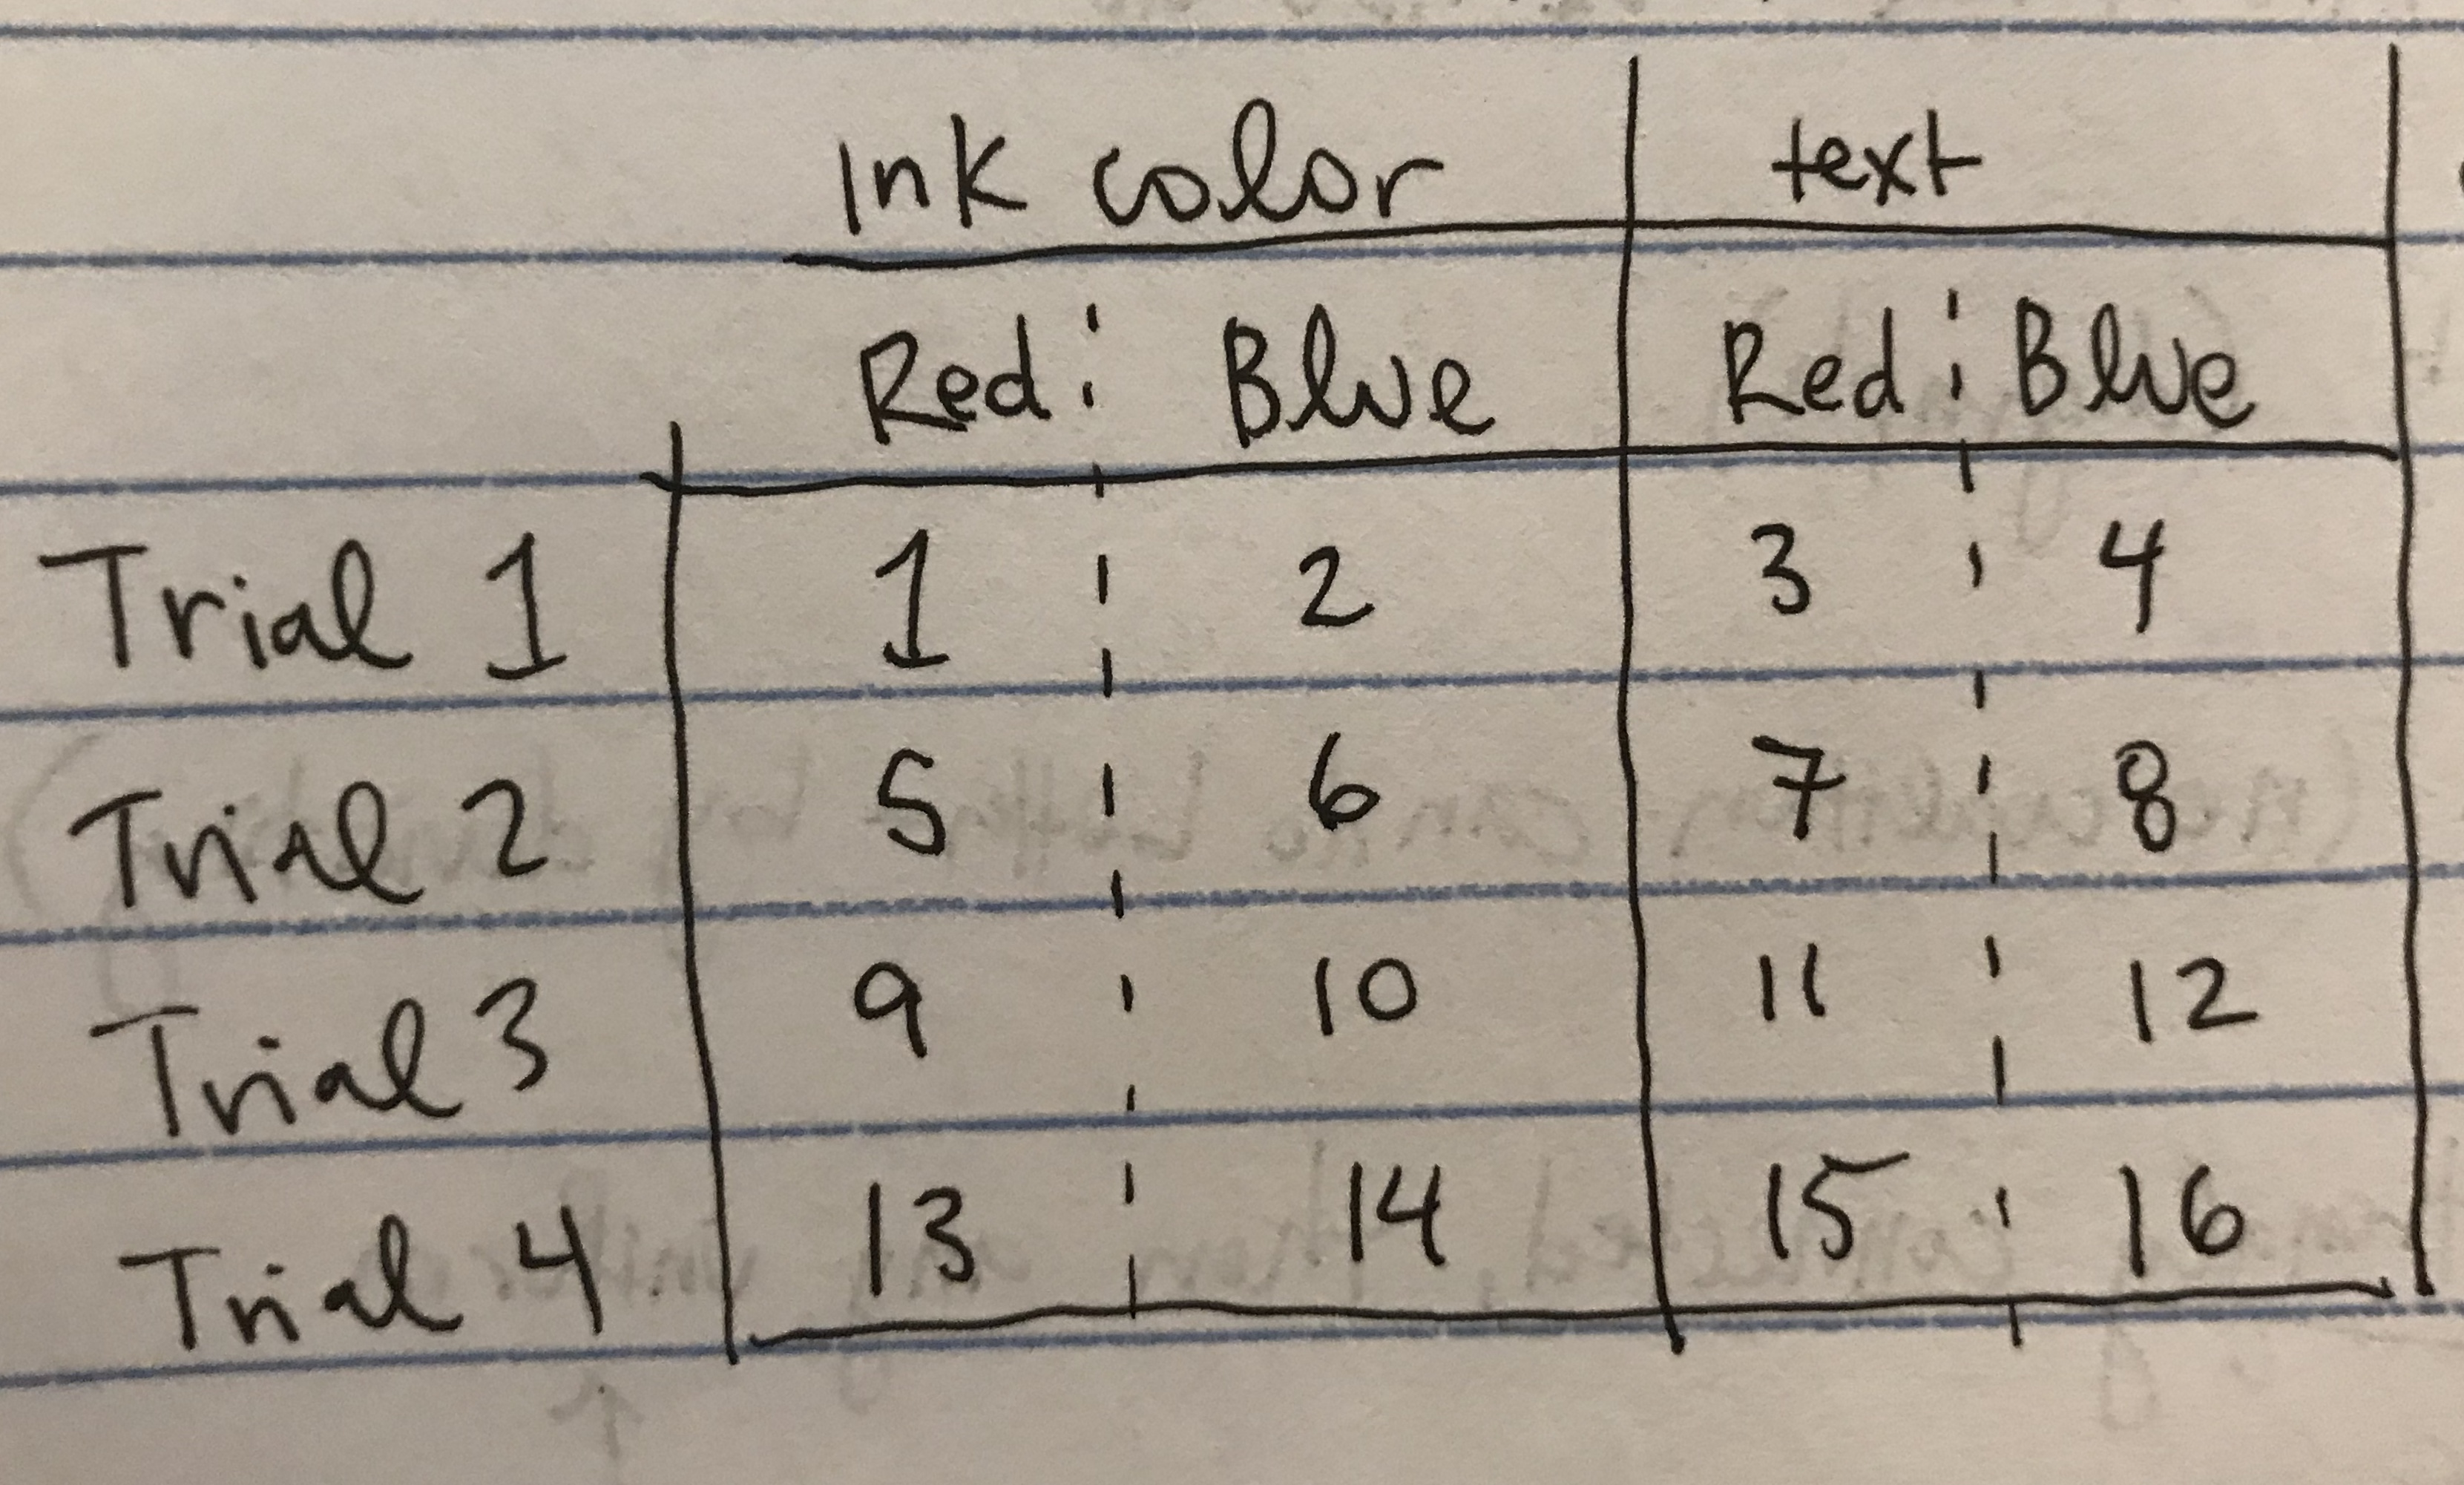
\includegraphics[origin=c,width=10cm]{encoding_strupe_vars}}
    \caption{Of the 24 possible orderings, the highlighted 8 satisfy the constraints.}%
    \label{fig:encoding_strupe_vars}%
\end{figure}

An experimental sequence consists of a specification for every trial in the experiment. Each trial is parameterized by factors, and the specification indicates which level of each factor is selected. Levels correspond naturally to boolean variables; a factor has one level at a time selected and each level can exist in either a selected state or a non-selected state.

The encoding we use allocates one boolean variable for each level of each factor of each trial. See figure \figref{encoding_strupe_vars} for a visualization of the variable allocation for the running Stroop example. In the running example, there are 4 trials, each of which is described by two factors with two levels. The encoding we use allocates one variable for every factor for every trial. As mentioned in the previous subsection, variables in the DIMACS CNF format are index-based, which means that the number 1 refers to the first boolean variable and so on. This means that the assignments to variables 1 through 4 represents the specification of the first trial. For instance, the assignment "1 -2 -3 4" means the ink color is red (and not blue), and the text is blue (and not red). For any experiment we allocate (total number of levels) * (number of trials) boolean variables which directly encode a specification of an experimental sequence.

\begin{figure}[t]
    \centerline{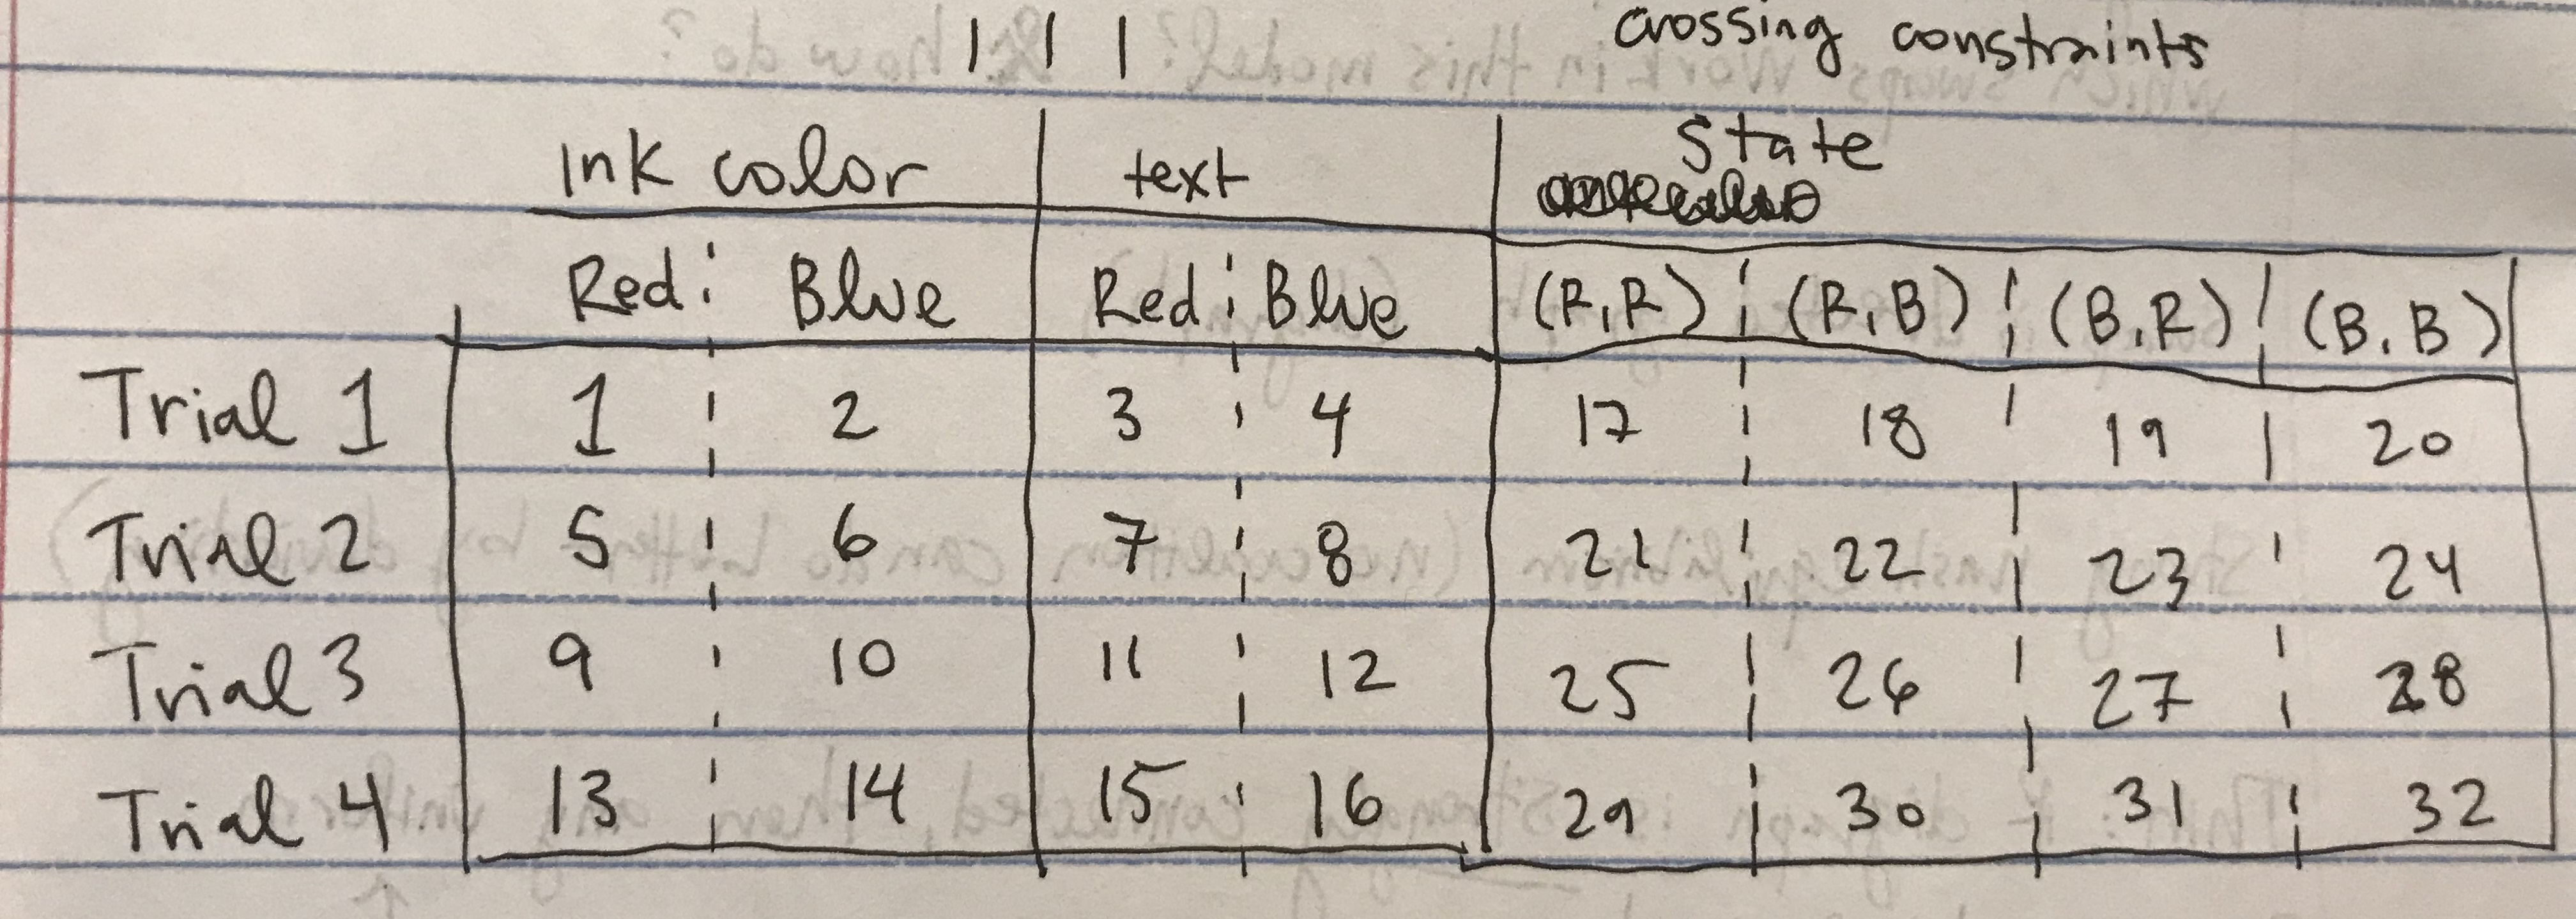
\includegraphics[origin=c,width=10cm]{stroop_crossing_vars}}
    \caption{Of the 24 possible orderings, the highlighted 8 satisfy the constraints.}%
    \label{fig:stroop_crossing_vars}%
\end{figure}


In addition to any user-defined constraints, we always have two kinds of constraints over the level variables to correctly model the experiment. The first are \emph{consistency constraints} which state that only one level of each factor is selected at once. In the running example constraints of the form "(1 and not 2) or (not 1 and 2)" for each pair of levels would ensure that only one level is true at a time. The second kind of constraint is a \emph{crossing constraint} which ensures that the correct number of each kind of possible trial occurs in the experimental sequences.

Representing crossing constraints is more complicated. In the running example, the logic for the crossing constraints should ensure that there is one (red ink, red text), one (red ink, blue text), one (blue ink, red text) and one (blue ink, blue text). To do encode this, we allocate 4 more variables for each trial, each of which literally encodes which of those 4 states that trial represents. See figure \figref{stroop_crossing_vars} for a visualization of the additional variables. Let's look at the constraints we need to add for the first trial-- first we'll add a constraint that specifies that trial is in the (red ink, red text) state if-and-only-if the red ink level is selected, and the red text level is selected (17 iff (1 and 3)). We add constraints of this form for the other 3 states as well, ie (18 iff (1 and 4)), (19 iff (2 and 3)), (20 iff (2 and 4)). Next, we create constraints to ensure that exactly one of each of the state variables across all the trials is true, ie, (exactly one of 17, 21, 25, 29 is true), (exactly one of 18, 22, 26, 30 is true), and so on. 


 TODO DIAGRAM.5

- as mentioned in the last chapter, levels correspond naturally to boolean values

- variables are index based (important for examples)

- keep track of : 1) variables which need assignemnts, 2) boolean formulas using those vars

- need additional constraint; one hot encoding, exactly one true at a time. literally represent as (a and not b) or (not a and b) -- this would be a bad choice if there were many levels but given the experimental size this is the best decision.

- walk through an example

- also need "sum" constraints. These also count up, but we expect these to be much bigger numbers, ie in the experiment w/ 7 factors w/ 2 levels, there are 64 of each level. So these we compile to "counting constraints". Basically these are linear inequality. We compile them to SAT efficeintly through the Tsietin transform (see next chapter for details).

- walk through an example

\subsection{Representing Derived Levels and Derivation Functions}

Internally, we pick out the levels, create new levels whose value depends on a boolean relationship of those levels. The relationship is then defined by a literal truth table:
- generate a truth table for the defined function by:
- each input is a factor
- then take all boolean combos and literally run it
- that generates a truth table
- encode that truth table in the logic by translating to CNF

- Work an example, for instance congruence.

\section{Communicating with the SAT-Sampler}

- block diagram of all runtime

- variables marked as "important" vs aux

- translate output to be human readable; easy to integrate with other environments


\section{Correctness Guarantees}

- cite guarantee from unigen

- postulate why this is preserved: TODO
